\documentclass{beamer}

% \usepackage{beamerthemesplit} // Activate for custom appearance
\usepackage{graphicx}

\setbeamertemplate{navigation symbols}{}
\setbeamertemplate{footline}
{
    \leavevmode%
    \hbox{%
        \begin{beamercolorbox}[wd=.333333\paperwidth,ht=2.25ex,dp=1ex,center]{author in head/foot}%
            \usebeamerfont{author in head/foot}\insertshortauthor
        \end{beamercolorbox}%
        \begin{beamercolorbox}[wd=.333333\paperwidth,ht=2.25ex,dp=1ex,center]{title in head/foot}%
            \usebeamerfont{title in head/foot}\insertshorttitle
        \end{beamercolorbox}%
        \begin{beamercolorbox}[wd=.333333\paperwidth,ht=2.25ex,dp=1ex,right]{date in head/foot}%
            \usebeamerfont{date in head/foot}\insertshortdate{}\hspace*{2em}
            \insertframenumber{} / \inserttotalframenumber\hspace*{2ex} 
        \end{beamercolorbox}}%
        \vskip0pt%
    }

\title{Kernel Panic}
\author{Gruppe 09}
\date{23.05.2019}

\begin{document}


{
\usebackgroundtemplate{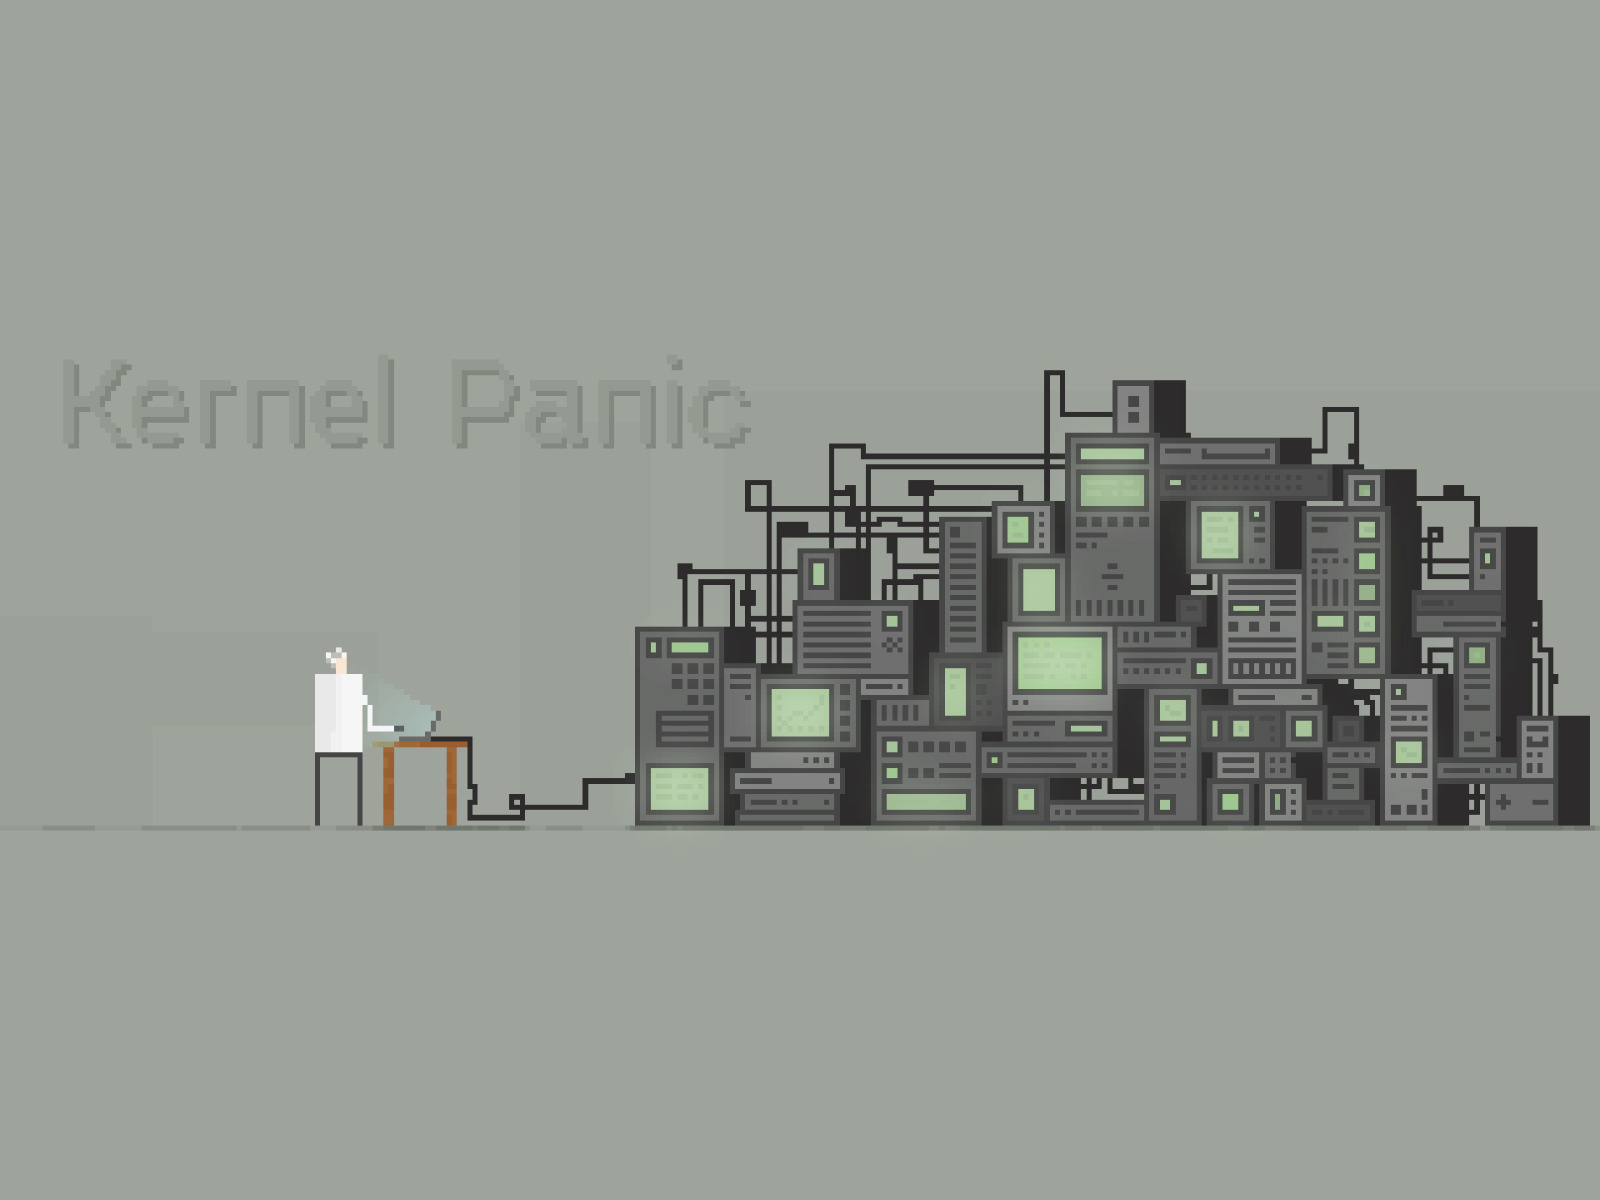
\includegraphics[width=\paperwidth]{kernel-panic-4-3.png}}
\frame{}
}

\section[Outline]{}
\frame{\tableofcontents}

\section{Spielkonzept}
\frame

\section{Spielende}
\frame

\section{Alleinstellungsmerkmal}
\frame

\section{Warum macht Kernel Panic Spaß?}
\frame

\end{document}
